\documentclass[12pt, oneside, titlepage]{article}   	% use "amsart" instead of "article" for AMSLaTeX format

\usepackage{graphicx}
\graphicspath{ {\string} }
\usepackage{subcaption}

%%%%%%%%%%%%%%%%%%%%%%%%%%%%%%%%%%%%%%%%%%%%%%%%%%%%
% set up packages
%%%%%%%%%%%%%%%%%%%%%%%%%%%%%%%%%%%%%%%%%%%%%%%%%%%%
\usepackage{geometry}                
\usepackage{textcomp}                
\usepackage{amsmath}                
\usepackage{graphicx}                
\usepackage{amssymb}                
\usepackage{fancyhdr}                
\usepackage{subcaption}                
\usepackage{bm}                
\usepackage{lineno}

\usepackage[superscript,noadjust]{cite} % puts dash in citations to abbreviate
\usepackage [autostyle, english = american]{csquotes} % sets US-style quotes

\usepackage{etoolbox} % block quotes

\usepackage{float}
\usepackage{color}

\usepackage{pgf}
\usepackage{tikz}
\usepackage{eqnarray}

\usepackage{listings} % code blocks
\usepackage{setspace}

\usepackage{lscape}

\usepackage{natbib}
%\bibliographystyle{abbrvnat}
\setcitestyle{authoryear,open={(},close={)},url=FALSE}

%%%%%%%%%%%%%%%%%%%%%%%%%%%%%%%%%%%%%%%%%%%%%%%%%%%%
% call packages
%%%%%%%%%%%%%%%%%%%%%%%%%%%%%%%%%%%%%%%%%%%%%%%%%%%%	
\geometry{letterpaper, marginparwidth=60pt} % sets up geometry              		
\linenumbers % adds line numbers 
\MakeOuterQuote{"} % sets quote style
\doublespacing % setspace

%%%%%%%%%%%%%%%%%%%%%%%%%%%%%%%%%%%%%%%%%%%%%%%%%%%%
% patches with etoolbox 
%%%%%%%%%%%%%%%%%%%%%%%%%%%%%%%%%%%%%%%%%%%%%%%%%%%%	
% block quotes
\AtBeginEnvironment{quote}{\small}

% linenumbers
\makeatletter
\patchcmd{\@startsection}{\@ifstar}{\nolinenumbers\@ifstar}{}{}
\patchcmd{\@xsect}{\ignorespaces}{\linenumbers\ignorespaces}{}{}
\makeatother

%%%%%%%%%%%%%%%%%%%%%%%%%%%%%%%%%%%%%%%%%%%%%%%%%%%%
% tikzlibrary modifications
%%%%%%%%%%%%%%%%%%%%%%%%%%%%%%%%%%%%%%%%%%%%%%%%%%%%	
\usetikzlibrary{fit}
\usetikzlibrary{positioning}
\usetikzlibrary{arrows}
\usetikzlibrary{automata}

%%%%%%%%%%%%%%%%%%%%%%%%%%%%%%%%%%%%%%%%%%%%%%%%%%%%
% page formatting; exact 1 in margins
%%%%%%%%%%%%%%%%%%%%%%%%%%%%%%%%%%%%%%%%%%%%%%%%%%%%
\pagestyle{plain}                                                     

\setlength{\textwidth}{6.5in}    
\setlength{\oddsidemargin}{0in}
\setlength{\evensidemargin}{0in}
\setlength{\textheight}{8.5in}
\setlength{\topmargin}{0in}
\setlength{\headheight}{0in}
\setlength{\headsep}{0in}
\setlength{\footskip}{.5in}

%%%%%%%%%%%%%%%%%%%%%%%%%%%%%%%%%%%%%%%%%%%%%%%%%%%%
% defining code blocks using listings package
%%%%%%%%%%%%%%%%%%%%%%%%%%%%%%%%%%%%%%%%%%%%%%%%%%%%

\definecolor{dkgreen}{rgb}{0,0.6,0}
\definecolor{gray}{rgb}{0.5,0.5,0.5}
\definecolor{mauve}{rgb}{0.58,0,0.82}

\lstset{frame=tb,
  language=R,
  aboveskip=3mm,
  belowskip=3mm,
  showstringspaces=false,
  columns=flexible,
  basicstyle={\small\ttfamily},
  numbers=none,
  numberstyle=\tiny\color{gray},
 % keywordstyle=\color{blue},
  commentstyle=\color{dkgreen},
  stringstyle=\color{mauve},
  breaklines=true,
  breakatwhitespace=true,
  tabsize=3,
  otherkeywords={0,1,2,3,4,5,6,7,8,9},
  deletekeywords={data,frame,length,as,character,dunif,ps},
}

%%%%%%%%%%%%%%%%%%%%%%%%%%%%%%%%%%%%%%%%%%%%%%%%%%%%
%%%%%%%%%%%%%%%%%%%%%%%%%%%%%%%%%%%%%%%%%%%%%%%%%%%%
% begin document
%%%%%%%%%%%%%%%%%%%%%%%%%%%%%%%%%%%%%%%%%%%%%%%%%%%%
%%%%%%%%%%%%%%%%%%%%%%%%%%%%%%%%%%%%%%%%%%%%%%%%%%%%

\begin{document}

\bibliographystyle{/Users/gregor/Dropbox/bibliography/styleFiles/ecology} 

%\section*{Appendix X}

\cite{cohen1966} developed a model to analyze bet hedging strategies in annual plants. A key feature of this model that distinguishes it from later work (\cite{ellner1985,ellner1985a}) is that it uses a density-independent fitness function. However, it's a helpful starting point because it introduces many of the characteristics that we're interested in understanding in our populations.

Cohen considered a discrete, unstructured model for an annual plant with a seed bank. Seeds in the seed bank germinate with probability $G$ or survive with a probability $S$. Of the seeds that germinate, the average number of seeds produced per germinated seedling is $Y$. The per capita reproductive success $Y$ is density-independent and assumed to be a random variable. Here, I will use a reparameterization (\cite{ellner1985a}). The population dynamics are given by 

\begin{align}
  \begin{split}
N(t+1) & = N(t) [ (1-G)S + G Y(t)] \\
N(t+1) & = N(t) \times S - N(t) \times SG + N(t) \times G Y(t)\\
  \end{split}
\end{align}

The long-term population growth rate for this model is the expectation of the geometric mean of the population growth rate

\begin{align}
  \begin{split}
\lim_{t \to \infty } \frac{\mathrm{log} N(t)}{t} = \sum_{i} P_i\mathrm{log}[(1-G)S + G Y_i] 
  \end{split}
\end{align}

where $P_i$ is the probability associated with a given $Y_i$.

Cohen's work frames bet hedging in the following terms. For a given distribution of fitness, amount of variation in fitness and seed survivorship, what germination fraction maximizes the long-term population growth rate? In the models developed by Cohen, the germination fraction that maximizes long-term population growth rate is a function of the distribution of fitness, the fitness values, and the rate of seed survivorship. Figure~\ref{fig:optimal_g} shows how these components interact, and how the optimal germination probability is depends on the distribution of fitness and seed survivorship. Specifically, the optimal germination probability ($G*$) is the $G$ that maximizes the geometric mean of the population growth rate (\cite{ellner1985a}).

I think that \cite{ellner1985a} (p. 101-103) has a good discussion of the predictions of the density-independent model. (1) Increasing the variance in fitness decreases the optimal germination probability (e.g. Figure~\ref{fig:variance}). (2) Increasing seed survivorship decreases the optimal germination probability (e.g Figure~\ref{fig:survivorship}). The degree to which increased seed survivorship decreases germination depends on the probability of a high fitness year. Specifically, as the probability of a high-fitness year decreases, the optimal germination probability decreases (e.g Figure ~\ref{fig:survivorship}). The behavior $G*$ near the limits as the probability of seed survivorship approaches 0 or 1 depends on the fitness values and distribution of fitness. (3) This is similar to the above, but an increase in the probability of a high-fitness year increases the optimal germination probability. (4) Finally, the model predicts that an increase in the mean fitness $Y$ leads to an increase in the optimal germination probability. I can't quite get the plots for this to work yet, which is why there is no figure for it. 

\bibliography{/Users/gregor/Dropbox/bibliography/seeds}

%
 \begin{figure}[h]
   \centering
  %#\begin{tabular}{@{}c@{\hspace{.5cm}}c@{}}
       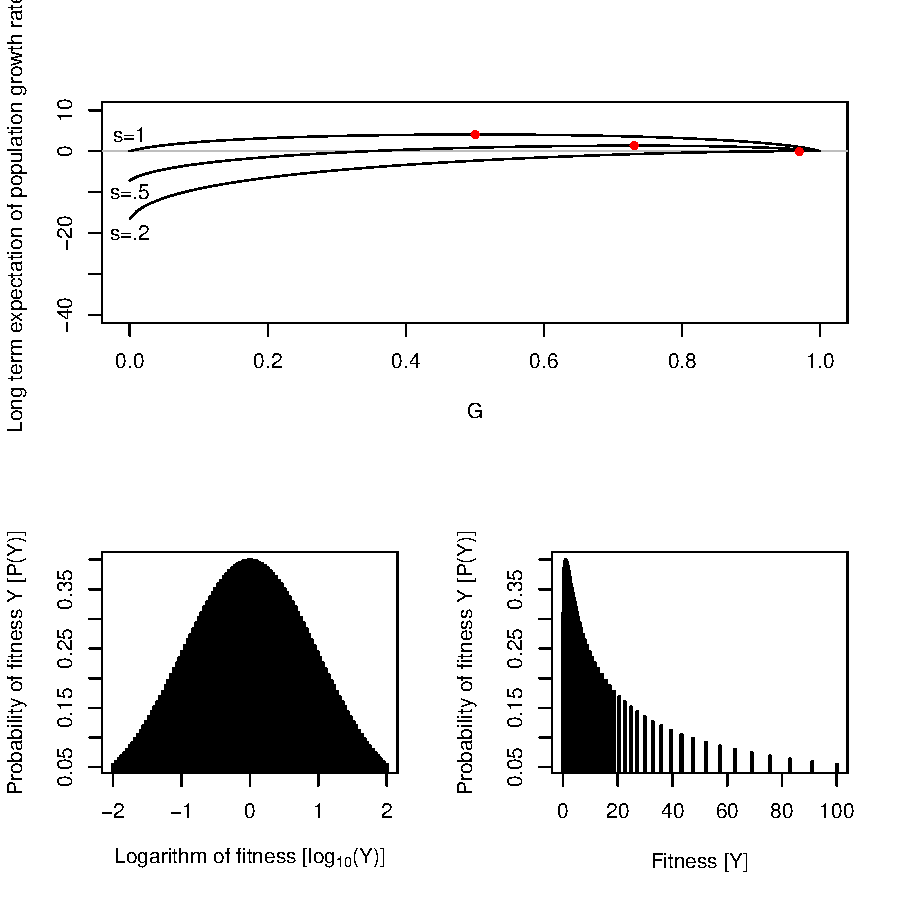
\includegraphics[page=1]{../figures/appendix-x-optimal.pdf}  
    \caption{ Expectation of the long-term population growth rate plotted as a function of germination probability (G) for several values of seed survivorship (s=1, .5, .2; equivalent to d=0,.5,.8 in Cohen 1966 Figure 7). In the top panel, the red points show the germination probability that maximizes population growth rate. The results are shown for a distribution of $P(Y_i)$ for which the distribution of log-10 fitness is normally distributed. The log-10 and untransformed discrete distributions for fitness are shown below.  }
 \label{fig:optimal_g}
\end{figure}
%
 \begin{figure}[h]
   \centering
  %#\begin{tabular}{@{}c@{\hspace{.5cm}}c@{}}
       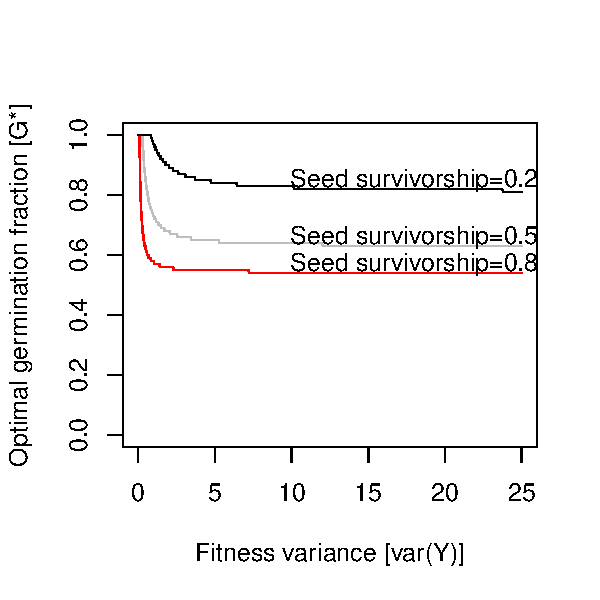
\includegraphics[page=1]{../figures/appendix-x-fitnessvariance.pdf}  
    \caption{ Increasing variance in fitness decreases the optimal germination fraction for a given level of seed survivorship. To generate this figure, I generated fitness distributions with the same mean but different variance and calculated the optimal germination fraction for each.  }
 \label{fig:variance}
\end{figure}
%
 \begin{figure}[h]
   \centering
  %#\begin{tabular}{@{}c@{\hspace{.5cm}}c@{}}
       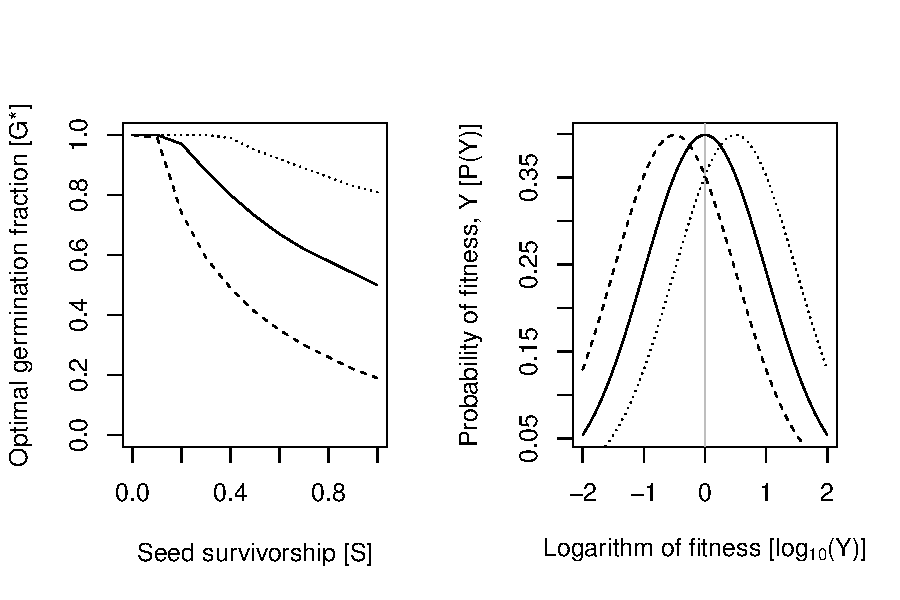
\includegraphics[page=1]{../figures/appendix-x-survivorship.pdf}  
    \caption{ Increasing seed survivorship (and thus decreasing the probability of seed decay) decreases the optimal germination fraction for a given distribution of fitness. The panel on the left shows the optimal germination fraction plotted against seed survivorship. Each line in the panel on the left corresponds to the distribution of fitness shown in the panel on the right. Together, the plots show that increasing seed survivorship and decreasing probabilities of high fitness years both decrease the optimal germination fraction. }
 \label{fig:survivorship}
\end{figure}



\end{document}